% Preamble: \usepackage{graphicx}
% Set \graphicspath to the directory containing the two PDF figures.
% figure* spans both columns in a two-column paper and also works in one column.

\begin{figure*}[t]
  \centering
  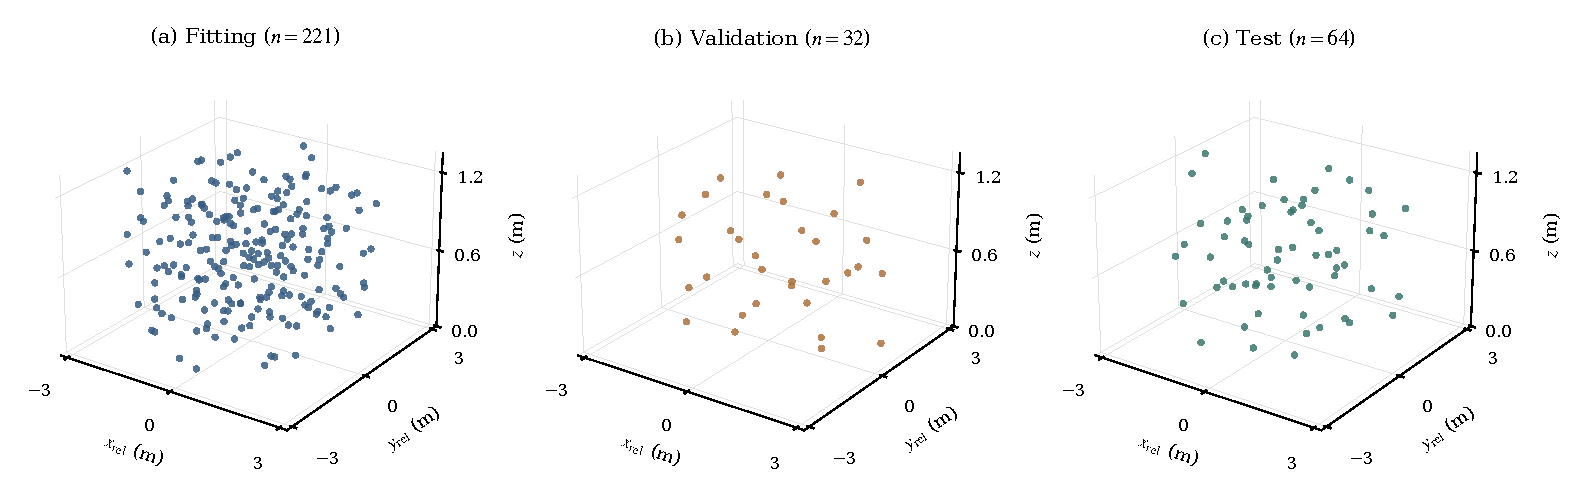
\includegraphics[width=\textwidth]{scenario_coverage.pdf}
  \caption{Target locations for the fitting, validation and test scenarios,
    expressed relative to the initial robot pose. The horizontal coordinates
    $x_{\mathrm{rel}}$ and $y_{\mathrm{rel}}$ point forward and left,
    respectively; $z$ is world height. Each point represents one scenario.
    All panels use the same coordinate limits and viewpoint; the vertical
    scale is expanded for readability.}
  \label{fig:scenario-coverage}
\end{figure*}

\begin{figure*}[t]
  \centering
  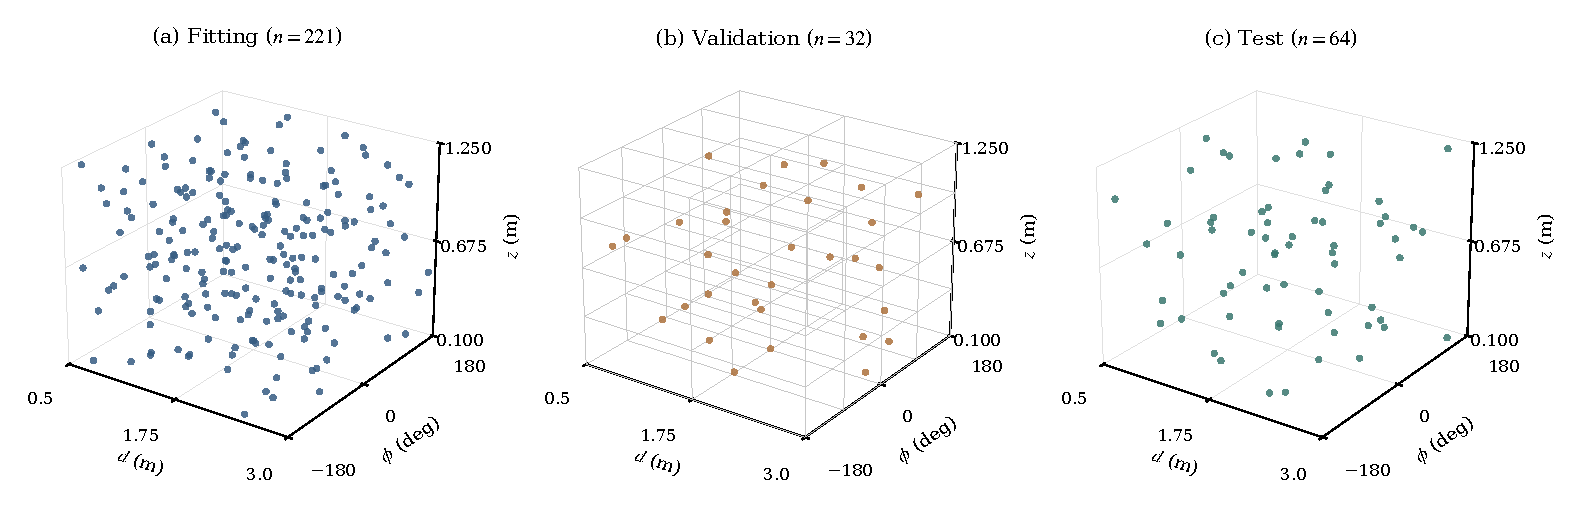
\includegraphics[width=\textwidth]{scenario_parameter_coverage_3d.pdf}
  \caption{Scenario coverage in target distance $d$, relative azimuth $\phi$
    and world height $z$. The lattice in panel~(b) partitions the parameter
    space into $2\times4\times4=32$ strata, with one validation scenario per
    stratum. Azimuths $-180^{\circ}$ and $180^{\circ}$ denote the same
    direction. These views show three of the six sampled parameters.}
  \label{fig:scenario-strata}
\end{figure*}
